\chapter{Resultados}   
\minitoc

\section{Comparaci\'on de propiedades \'opticas entre sistemas moleculares dipolar, cuadrupolar y octopolar}

Inicialmente se prepararon soluciones en THF y suspensiones acuosas de nanopart\'iculas para las mol\'eculas 1NDS, 2NQS y 3NOS (Ver Figura \ref{ar2}) a una concentraci\'on de $6.25 \times 10^{-6}$ utilizando CTAB. En la figura \ref{X} se muestran los espectros de absorci\'on lineal molar $\epsilon$ de estas soluciones y suspensiones. La mayor absorci\'on se presenta en el sistema octopolar, posteriormente en el sistema cuadrupolar y finalmente en el sistema dipolar. 

\begin{figure}[h]
\centering
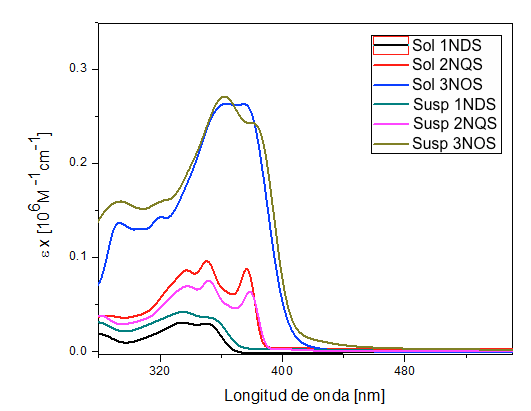
\includegraphics[width=0.85\textwidth]{resultados/sec1/comp}
\caption{Espectros de absorci\'on molar de 1NDS, 2NQS, 3NOS. Las etiquetas \emph{sol} y \emph{susp} se refieren a los sistemas moleculares en soluci\'on y suspensi\'on respectivamente}\label{X}
\end{figure}

Posteriormente se adquirieron los espectros de emisi\'on lineal de las soluciones y suspensiones a la misma concentraci\'on, utilizando un diodo l\'aser de 370 $nm$. Estos espectros se muestran en la figura \ref{eslia} y se puede apreciar que la mayor emisi\'on se presenta en el sistema octopolar en soluci\'on y luego en suspensi\'on de nanopart\'iculas. Sin embargo en todos los sistemas moleculares, la emisi\'on del material en soluci\'on es mayor que en suspensi\'on de nanopart\'iculas y adem\'as, cada sistema molecular en suspensi\'on puede sufrir modificaciones estructurales; el caso mas notorio fue el del sistema octopolar 3NOS, cuyo espectro de emisi\'on en suspensi\'on sufri\'o un corrimiento hacia el rojo comparado con el espectro en soluci\'on (Ver Figura \ref{3nsolsusp}).



\begin{figure}
\centering
\begin{subfigure}{\textwidth}
\centering
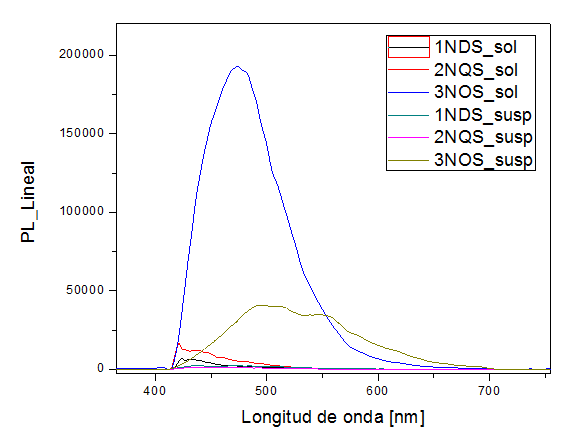
\includegraphics[width=0.8\textwidth]{resultados/sec1/emilinealtodas}
\caption{Espectros de emisi\'on lineal de 1NDS, 2NQS y 3NOS en soluci\'on y suspensi\'on de nanopart\'iculas}\label{eslia}
\end{subfigure}
\begin{subfigure}{\textwidth}
\centering
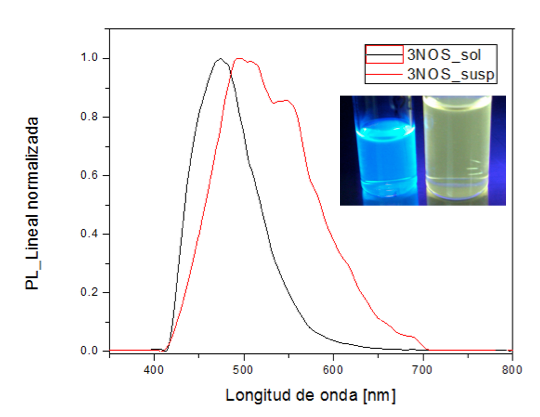
\includegraphics[width=0.8\textwidth]{resultados/sec1/emilinealnorm3N}
\caption{Espectros normalizados y fluorescencia visible de 3NOS en soluci\'on (azul) y suspensi\'on (amarilla) }\label{3nsolsusp}
\end{subfigure}
\caption{Espectros de emisi\'on lineal de 1NDS, 2NQS y 3NOS}
\label{ghghh}
\end{figure}

En comparaci\'on con el sistema octopolar, la emisi\'on lineal (y no lineal como se ver\'a en seguida) de los sistemas dipolar y cuadrupolar fue muy escasa. Por ello \'unicamente fue de inter\'es medir varias veces la eficiencia cu\'antica de fluorescencia del sistema octopolar 3NOS, inicialmente en soluci\'on y suspensi\'on acuosa de nanopart\'iculas utilizando CTAB, nuevamente a una concentraci\'on de $6.25 \times 10^{-6}$; los valores obtenidos, utilizando la ecuaci\'on \ref{final}, se muestran en la tabla \ref{tablita}. 

Se realizaron tres y cinco mediciones de eficiencia cu\'antica de fluorescencia del sistema octopolar en soluci\'on y suspensi\'on respectivamente; adem\'as se realiz\'o una correcci\'on al valor de eficiencia promedio obtenido para la soluci\'on, debido a que la sensibilidad de respuesta del PMT no es la misma para todas las longitudes de onda. Cuando la fluorescencia de la muestra de inter\'es y de la referencia (Rodamina 6G) tienen longitudes de onda similares, el PMT responder\'a de la misma manera en ambas muestras; sin embargo, si la muestra y la referencia emiten a diferentes longitudes de onda, es necesario introducir un factor de correci\'on. En el caso de la soluci\'on octopolar dicho factor fue de 0.6.

\begin{table}[H]
\centering
\scalebox{0.82}{
\begin{tabular}{| l | c | c | c | c | c | c | c | c | r | }  %p{6.5cm} | c |
\hline
 3NOS           & $\Phi_1$	&$\Phi_2$ &$\Phi_3$&$\Phi_4$&$\Phi_5$& $\Phi_{Promedio}$&$\Phi_{Promedio}$ /correcci\'on PMT  \\ \hline   %\multicolumn{8}{|c|}
Soluci\'on &    0.457&	0.539& 0.341	& -	& -	&0.44& 0.26 \\ \hline
Suspensi\'on & 	0.129 &	 0.191& 0.094 & 0.225& 0.226	& 0.17&0.17 \\ \hline
\end{tabular} } 
\caption{ Valores obtenidos de eficiencia cu\'antica de fluorescencia $\Phi$ para el sistema octopolar  \label{tablita}}
\end{table}


Las mediciones iniciales de $\sigma^{TPA}$ en el rango de 740 $nm$ a 840 $nm$ para los tres sistemas moleculares se realizaron a una concentraci\'on de $6.25\times 10^{-6} M$. A esta concentraci\'on los espectros de emisi\'on no lineal de los sistemas dipolar y cuadrupolar tanto en soluci\'on como en suspensi\'on no pudieron visualizarse (Ver Figura \ref{nel}); sin embargo, los espectros del sistema octopolar en soluci\'on y suspensi\'on, para algunas longitudes de onda de excitaci\'on, se muestran en la figura \ref{sip}.

Para calcular la secci\'on transversal de absorcion de dos fotones en este rango con la t\'ecnica de TPEF se utiliz\'o la ecuaci\'on \ref{finalsigma}, sin embargo, como los espectros de emisi\'on no lineal de la muestra de inter\'es y de referencia se adquirieron bajo las mismas condiciones, entonces la eficiencia de colecci\'on de fluorescencia es constante y $\eta_{ref}=\eta$; de igual manera, la potencia incidente fue la misma para todas las muestras $\langle P(t)\rangle_{ref}=\langle P(t)\rangle$. Asumiendo que $n_{ref}/n\approx 1$, el par\'ametro a calcular para conocer $\sigma^{TPA}$ es el valor de la integral del espectro de emisi\'on no lineal de la referencia y de la muestra de inter\'es $\langle F(t)\rangle_{ref}$ y $\langle F(t)\rangle$; los resultados obtenidos para la mol\'ecula octopolar 3NOS se muestran en la gr\'afica de la figura \ref{tpaprimeros}.

\begin{figure}
\centering
\begin{subfigure}{\textwidth}
\centering
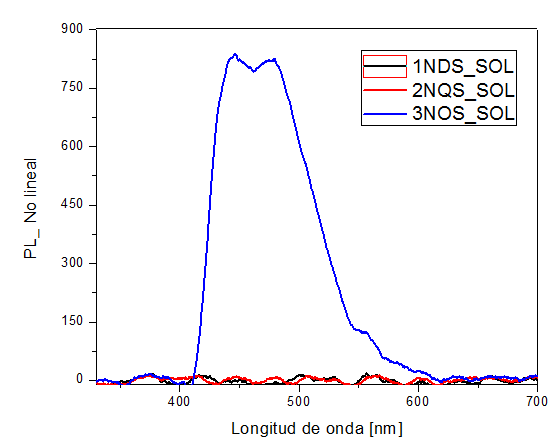
\includegraphics[width=0.6\textwidth]{resultados/sec1/nojalo}
\caption{Espectros de emisi\'on no lineal para 1NDS, 2NQS y 3NOS en soluci\'on con un haz de excitaci\'on a 760 $nm$ }\label{nel}
\end{subfigure}
\begin{subfigure}{\textwidth}
\centering
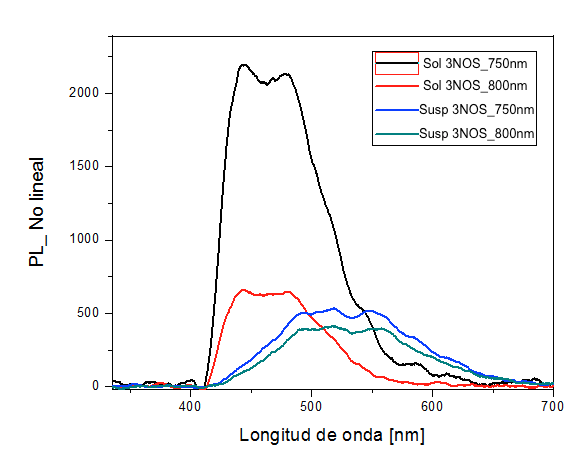
\includegraphics[width=0.7\textwidth]{resultados/sec1/sijalo}
\caption{Comparaci\'on de espectros de emisi\'on no lineal para 3NOS en soluci\'on y suspensi\'on para diferentes longitudes de onda de excitaci\'on }\label{sip}
\end{subfigure}
\caption{Espectros de emisi\'on no lineal}
\label{ghghh}
\end{figure}

\begin{figure}[h]
\centering
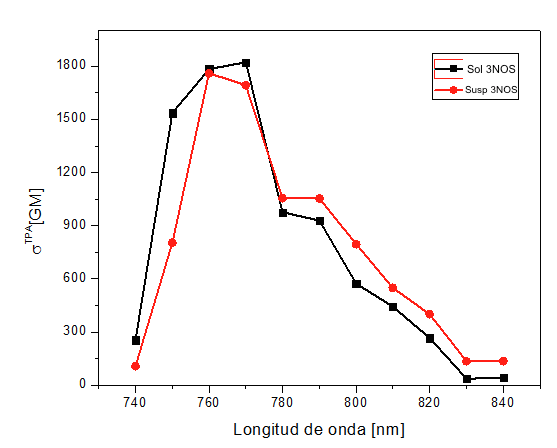
\includegraphics[width=0.7\textwidth]{resultados/sec1/TPA_1}
\caption{Espectro de absorci\'on no lineal de 3NOS en soluci\'on y suspensi\'on}\label{tpaprimeros}
\end{figure}

Posteriormente se realizaron pruebas para recubrir las nanopart\'iculas de la mol\'ecula octopolar con PEG 5000 sin utilizar surfactantes. Se prepar\'o una suspensi\'on acuosa de nanopart\'iculas a una concentraci\'on de $6.43 \times 10^{-6}M$, utilizando una concentraci\'on de PEG 5000 de $5\times 10^{-6} M$. En la figura \ref{grr} se muestra una comparaci\'on de los espectros de absorci\'on (\ref{abspeg1}) y emisi\'on lineal (\ref{emipeg1}) de la mol\'ecula octopolar en soluci\'on, suspensi\'on utilizando CTAB y suspensi\'on de nanopart\'iculas utilizando PEG 5000, todas a la misma concentraci\'on $6.43 \times 10^{-6}M$. 

\begin{figure}
\centering
\begin{subfigure}{0.5\textwidth}
\centering
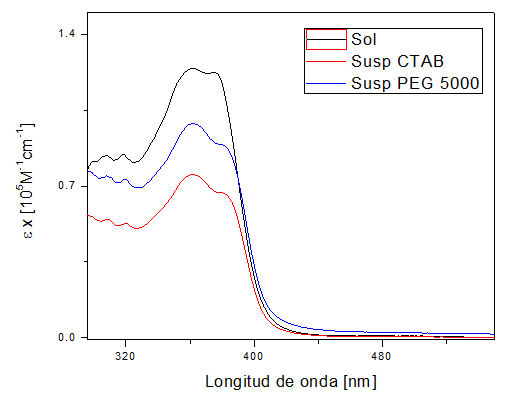
\includegraphics[width=\textwidth]{resultados/sec1/abs_peg5000}
\caption{Absorci\'on molar lineal }\label{abspeg1}
\end{subfigure}
\begin{subfigure}{0.49\textwidth}
\centering
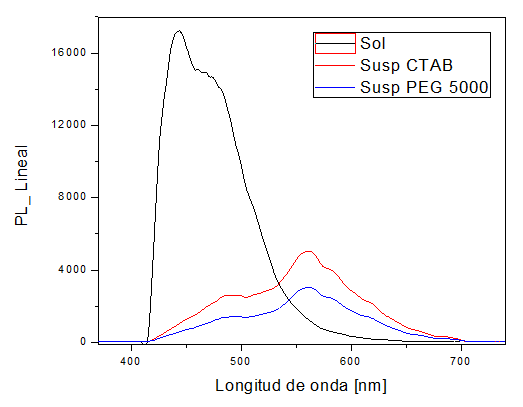
\includegraphics[width=\textwidth]{resultados/sec1/emi_peg5000}
\caption{Emisi\'on lineal }\label{emipeg1}
\end{subfigure}
\caption{Espectros de la mol\'ecula octopolar en soluci\'on \emph{Sol} y  en suspensiones con CTAB \emph{Susp CTAB} y PEG \emph{Susp PEG 5000}}
\label{grr}
\end{figure}

Se realizaron cinco mediciones de eficiencia cu\'antica de fluorescencia para la suspensi\'on acuosa de nanopart\'iculas funcionalizadas con PEG 5000 obteniendo una eficiencia promedio $\Phi_{Promedio}$ de 0.14. Tambi\'en se midi\'o la secci\'on transversal de absorci\'on de dos fotones de esta suspensi\'on para las siguientes longitudes de onda de excitaci\'on: 760, 780, 800 y 815 $nm$; los valores de $\sigma^{TPA}$ para la mol\'ecula octopolar en soluci\'on, suspensi\'on con CTAB y suspensi\'on con PEG 5000 se muestran en la gr\'afica de la figura \ref{valoressigmapeg1}.

\begin{figure}[h]
\centering
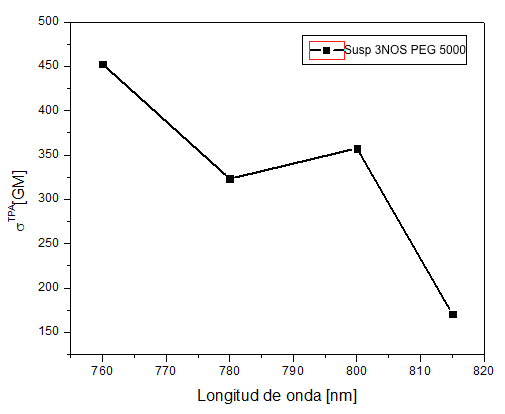
\includegraphics[width=0.7\textwidth]{resultados/sec1/TPA_PEG1}
\caption{Espectro de absorci\'on no lineal para 3NOS en soluci\'on \emph{Sol} y suspensiones con CTAB \emph{Susp CTAB} y PEG 5000, \emph{Susp PEG 5000}}\label{valoressigmapeg1}
\end{figure}

En este trabajo la mol\'ecula octopolar fue uno de los sistemas moleculares  de mayor inter\'es, por ello se determinaron los valores de $\sigma^{TPA}$ en el rango de longitudes de onda incidentes de 650 a 760 $nm$ implementando el arreglo \'optico de TPEF como se explic\'o en la secci\'on \ref{laserchidote}. En este rango se determin\'o $\sigma^{TPA}$ para la mol\'ecula 3NOS en soluci\'on a una concentraci\'on de $6.43 \times 10^{-6} M$; sin embargo, debido a la sensibilidad del arreglo, algunos espectros de emisi\'on no lineal no pudieron visualizarse a ciertas longitudes de onda y por lo tanto tampoco se pudo determinar $\sigma^{TPA}$. Los resultados se muestran en la figura \ref{valoressigmafs} junto con los resultados obtenidos anteriormente para la soluci\'on en el primer rango, de 740 a 840 $nm$ (Ver Figura \ref{tpaprimeros}).

\begin{figure}[h]
\centering
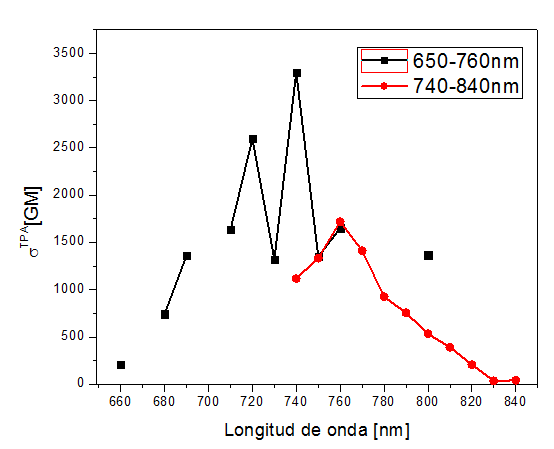
\includegraphics[width=0.7\textwidth]{resultados/sec1/TPA_femto}
\caption{Espectros de absorci\'on no lineal para 3NOS en soluci\'on de 650--760 nm y de $740-840nm$}\label{valoressigmafs}
\end{figure}

Posteriormente se realiz\'o una funcionalizaci\'on de nanopart\'iculas de la mol\'ecula octopolar, utilizando ahora el PEG 2000. Se prepar\'o una suspensi\'on acuosa de nanopart\'iculas sin CTAB a una concentraci\'on de $6.43 \times 10^{-6} M$ y con una concentraci\'on de PEG 2000 en la suspensi\'on de $6\times 10^{-4} M$. En la figura \ref{temi} se muestran un par de im\'agenes de esta suspensi\'on adquiridas con un microscopio electr\'onico de transmisi\'on o TEM por sus siglas en ingles, de la marca Philips modelo XL ; los di\'ametros de las nanopart\'iculas van de 16.8 a 33.7 $nm$. 

\begin{figure}[h]
\centering
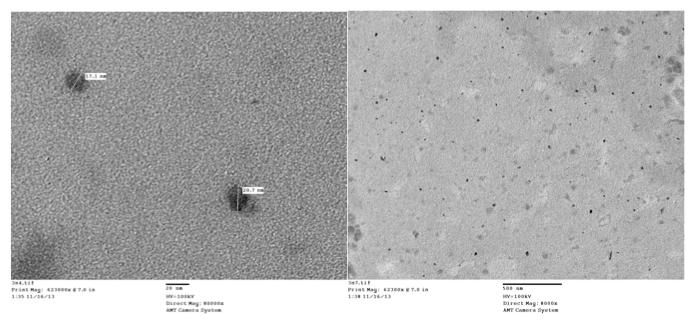
\includegraphics[width=\textwidth]{resultados/sec1/tem}
\caption{Im\'agenes TEM con escala de 20 y 500 $nm$}\label{temi}
\end{figure}

El PEG 2000 facilita la funcionalizaci\'on de nanopart\'iculas porque tiene m\'as grupos funcionales que el PEG 5000 como se mencion\'o en la secci\'on \ref{pegis}, adem\'as las suspensiones fabricadas con PEG 2000 fueron m\'as estables; en un tiempo de almacenamiento de m\'as de cinco meses a temperatura ambiente la suspensi\'on de nanopart\'iculas de 3NOS no se precipit\'o. Por ello y por las propiedades \'opticas que present\'o la mol\'ecula octopolar se decidi\'o internalizar esta suspensi\'on acuosa de nanopart\'iculas funcionalizadas con PEG 2000 en la l\'inea celular X.

Se internalizaron 500 $\mu l$ de la suspensi\'on a una concentraci\'on de $6.43 \times 10^{-6} M$ ...  



